\title{Monografia - LUARKIAN}

\documentclass[
	% -- opções da classe memoir --
	12pt,				% tamanho da fonte
    oneside,			% Tipo de impressão, frente-verso(twoside) ou apenas frente(oneside)
	a4paper,			% tamanho do papel. 
	% -- opções da classe abntex2 --
	chapter=TITLE,		% títulos de capítulos convertidos em letras maiúsculas
	% -- opções do pacote babel --    
	english,			% idioma adicional para hifenização
	brazil				% o último idioma é o principal do documento    
	]{abntex2}
    
    %\renewcommand{\ABNTEXpartfontsize}{\normalsize}
	%\renewcommand{\ABNTEXchapterfontsize}{ \large}
	%\renewcommand{\ABNTEXsectionfontsize}{\normalsize}
	%\renewcommand{\ABNTEXsubsectionfontsize}{\normalsize}

% ---
% Pacotes básicos 
% ---
\usepackage{lmodern}			% Usa a fonte Latin Modern			
\usepackage[T1]{fontenc}		% Selecao de codigos de fonte.
\usepackage[utf8]{inputenc}		% Codificacao do documento (conversão automática dos acentos)
\usepackage{lastpage}			% Usado pela Ficha catalográfica
\usepackage{indentfirst}		% Indenta o primeiro parágrafo de cada seção.
\usepackage{color}				% Controle das cores
\usepackage{graphicx}			% Inclusão de gráficos
\usepackage{microtype} 			% para melhorias de justificação
\usepackage{todonotes}
\usepackage{tabularx}


\definecolor{algColor}{RGB}{255,206,206} % rgb(255, 206, 206)

% Pacotes para algoritmos/pseudo-código
\usepackage{listings}

\renewcommand{\lstlistingname}{Programa}

\lstset
{ %Formatting for code in appendix
    language=C,
    basicstyle=\footnotesize,
    numbers=left,
    stepnumber=1,
    frame = single,
    showstringspaces=false,
    tabsize=2,
    breaklines=true,
    xleftmargin=10pt,
    breakatwhitespace=false,
    extendedchars=true,
    literate={á}{{\'a}}1 
             {ã}{{\~a}}1
             {é}{{\'e}}1
             {í}{{\'i}}1
             {õ}{{\~o}}1
             {ç}{{\c{c}}}1,
}

\renewcommand{\lstlistlistingname}{Lista de códigos}

% Configura a ``Lista de Códigos'' conforme as regras da ABNT (para abnTeX2)
\begingroup\makeatletter
\let\newcounter\@gobble\let\setcounter\@gobbletwo
  \globaldefs\@ne \let\c@loldepth\@ne
  \newlistof{listings}{lol}{\lstlistlistingname}
  \newlistentry{lstlisting}{lol}{0}
\endgroup

\renewcommand{\cftlstlistingaftersnum}{\hfill--\hfill}

\let\oldlstlistoflistings\lstlistoflistings
\renewcommand{\lstlistoflistings}{%
   \begingroup%
   \let\oldnumberline\numberline%
   \renewcommand{\numberline}{\lstlistingname\space\oldnumberline}%
   \oldlstlistoflistings%
   \endgroup}
% ---
% Pacotes adicionais, usados apenas no âmbito do Modelo Canônico do abnteX2
% ---
\usepackage{lipsum}				% para geração de dummy text
% ---


% ---
% Pacotes de citações
% ---
%\usepackage[brazilian,hyperpageref]{backref}	 % Paginas com as citações na bibl
\usepackage[alf, abnt-etal-cite=2]{abntex2cite}	% Citações padrão ABNT

% --- 
% CONFIGURAÇÕES DE PACOTES
% --- 

\usepackage{abntex_ufrr_dcc}


% PACOTES DE ALGORITMO

\usepackage{algpseudocode,algorithm}
% Declaracoes em Português

\algrenewcommand\algorithmicend{\textbf{FIM}}
\algrenewcommand\algorithmicdo{\textbf{FAÇA}}
\algrenewcommand\algorithmicwhile{\textbf{ENQUANTO}}
\algrenewcommand\algorithmicfor{\textbf{PARA}}
\algrenewcommand\algorithmicforall{\textbf{PARA TODO}}
\algrenewcommand\algorithmicif{\textbf{SE}}
\algrenewcommand\algorithmicthen{\textbf{ENTÃO}}
\algrenewcommand\algorithmicelse{\textbf{SENÃO}}
\algrenewcommand\algorithmicreturn{\textbf{RETORNE}}
\algrenewcommand\algorithmicfunction{\textbf{FUNÇÃO}}
% New definitions
\algnewcommand\algorithmicswitch{\textbf{ESCOLHA}}
\algnewcommand\algorithmiccase{\textbf{CASO}}
\algnewcommand\algorithmicassert{\texttt{assert}}
\algnewcommand\Assert[1]{\State \algorithmicassert(#1)}%
% New "environments"
\algdef{SE}[SWITCH]{Switch}{EndSwitch}[1]{\algorithmicswitch\ #1\ \algorithmicdo}{\algorithmicend\ \algorithmicswitch}%
\algdef{SE}[CASE]{Case}{EndCase}[1]{\algorithmiccase\ #1}{\algorithmicend\ \algorithmiccase}%
\algtext*{EndSwitch}%
\algtext*{EndCase}%


% Rearranja os finais de cada estrutura
\algrenewtext{EndWhile}{\algorithmicend\ \algorithmicwhile}
\algrenewtext{EndFor}{\algorithmicend\ \algorithmicfor}
\algrenewtext{EndIf}{\algorithmicend\ \algorithmicif}
\algrenewtext{EndFunction}{\algorithmicend\ \algorithmicfunction}

% O comando For, a seguir, retorna 'para #1 -- #2 até #3 faça'
\algnewcommand\algorithmicto{\textbf{até}}
\algrenewtext{For}[3]%
{\algorithmicfor\ #1 $\gets$ #2 \algorithmicto\ #3 \algorithmicdo}


% ---
% Configurações do pacote backref
% Usado sem a opção hyperpageref de backref
%\renewcommand{\backrefpagesname}{Citado na(s) página(s):~}
% Texto padrão antes do número das páginas
%\renewcommand{\backref}{}
% Define os textos da citação
%\renewcommand*{\backrefalt}[4]{
%	\ifcase #1 %
%		Nenhuma citação no texto.%
%	\or
%		Citado na página #2.%
%	\else
%		Citado #1 vezes nas páginas #2.%
%	\fi}%
% ---

% ---
% Informações de dados para CAPA e FOLHA DE ROSTO
% ---
\titulo{A DEFINIR}

\autor{LUARKIAN KAYPE DE SOUSA}
\local{Boa Vista - RR}
\data{2018}
\orientador{Dr. Herbert Oliveira Rocha}

\tipotrabalho{Monografia}

\preambulo{Monografia de Graduação apresentada ao Departamento de Ciência da Computação da Universidade Federal de Roraima como requisito parcial para a obtenção do grau de Bacharel em Ciência da Computação.}

%Trabalho de conclusão de curso  na área de Verificação de Software desenvolvido na UFRR com o %objetivo \textcolor{red}{VERIFICAR O PADRÃO DOS OUTROS TCC} de gerar casos de teste para %sistemas embarcados críticos	

% ---

%-- Informações de dado para a FOLHA DE APROVAÇÃO
\renewcommand{\dataDefesa}{A DEFINIR}
\renewcommand{\orientadorBanca}{Prof. Dr. Herbert Oliveira Rocha}
\renewcommand{\primeiroMembroBanca}{Prof. MSc. Felipe Leite Lobo}
\renewcommand{\segundoMembroBanca}{Prof. MSc. Miguel Raymundo Flores Santibañez}

% ---
% Configurações de aparência do PDF final

% alterando o aspecto da cor azul
\definecolor{blue}{RGB}{41,5,195}

% informações do PDF
\makeatletter
\hypersetup{
     	%pagebackref=true,
		pdftitle={\@title}, 
		pdfauthor={\@author},
    	pdfsubject={\imprimirpreambulo},
	    pdfcreator={LaTeX with abnTeX2},
		pdfkeywords={abnt}{latex}{abntex}{abntex2}{trabalho acadêmico}, 
		colorlinks=true,       		% false: boxed links; true: colored links
    	linkcolor=blue,          	% color of internal links
    	citecolor=blue,        		% color of links to bibliography
    	filecolor=magenta,      	% color of file links
		urlcolor=blue,
		bookmarksdepth=4
}
\makeatother
% --- 

% --- 
% Espaçamentos entre linhas e parágrafos 
% --- 

% O tamanho do parágrafo é dado por:
\setlength{\parindent}{1.3cm}

% Controle do espaçamento entre um parágrafo e outro:
\setlength{\parskip}{0.2cm}  % tente também \onelineskip

% ---
% compila o indice
% ---
\makeindex
% ---

% ----
% Início do documento
% ----
\begin{document}

% Retira espaço extra obsoleto entre as frases.
\frenchspacing 

% ----------------------------------------------------------
% ELEMENTOS PRÉ-TEXTUAIS
% ----------------------------------------------------------
% \pretextual

% ---
% Capa
% ---
\imprimircapa
% ---

% ---
% Folha de rosto
% (o * indica que haverá a ficha bibliográfica)
% ---
\imprimirfolhaderosto
% ---

% ---
% Inserir folha de aprovação
% ---
\imprimirfolhadeaprovacao
% ---
% Dedicatória
% ---
\begin{dedicatoria}
   \vspace*{\fill}
   \centering
   \noindent
   \textit{Fazer dedicatória} \vspace*{\fill}
\end{dedicatoria}
% ---

% ---
% Agradecimentos
% ---
\begin{agradecimentos}
Fazer agradecimentos!!

\end{agradecimentos}
% ---

% ---
% Epígrafe
% ---
\begin{epigrafe}
    \vspace*{\fill}
	\begin{flushright}
		\textit{Procurar frase massa!!}
	\end{flushright}
\end{epigrafe}
% ---

% ---
% RESUMOS
% ---

% resumo em português
\setlength{\absparsep}{18pt} % ajusta o espaçamento dos parágrafos do resumo
\begin{resumo}
Fazer resumo!!

 \vspace{\onelineskip}
 
 \noindent 
 \textbf{Palavras-chaves}: ??
\end{resumo}

\begin{resumo}[Abstract]
 \begin{otherlanguage*}{english}
   Fazer Abstract!!

   \vspace{\onelineskip}
 
   \noindent 
   \textbf{Key-words}: ??
 \end{otherlanguage*}
\end{resumo}
% ---
% inserir lista de ilustrações
% ---
\pdfbookmark[0]{\listfigurename}{lof}
\listoffigures*
\cleardoublepage
% ---

% ---
% inserir lista de tabelas
% ---
\pdfbookmark[0]{\listtablename}{lot}
\listoftables*
\cleardoublepage
% ---

% ---
% inserir lista de abreviaturas e siglas
% ---
\begin{siglas}
  \item[GPS] Global Positioning System
  \item[RFID] Radio Frequency Identification
  \item[RSSI] Received Signal Strength Indication
  \item[RTLS] Real Time Location System
  \item[WLAN] Wireless Local Area Network
  \item[UML]  Unified Modeling Language

\end{siglas}
% ---

% ---
% inserir lista de símbolos
% ---
% \begin{simbolos}  
%   \item[$ \Gamma $] \todo{Atualizar esta lista!} Letra grega Gama
%   \item[$ \Lambda $] Lambda
%   \item[$ \zeta $] Letra grega minúscula zeta
%   \item[$ \in $] Pertence
% \end{simbolos}
% % ---

% ---
% inserir o sumario
% ---
\pdfbookmark[0]{\contentsname}{toc}
\tableofcontents*
\cleardoublepage
% ---



% ----------------------------------------------------------
% ELEMENTOS TEXTUAIS
% ----------------------------------------------------------
\textual
% ----------------------------------------------------------
% Introdução
% ----------------------------------------------------------
\chapter{INTRODUÇÃO}


%===========================================================
%INTRODUÇÃO
%===========================================================
A localização é um tipo de informação situacional muito importante, no contexto geral temos aplicações que fornecem a
localização de algo, por exemplo para casas nós temos ruas, número da casa, e bairro. No sistema de posicionamento global
para um ponto temos latitude e longitude. Entretanto quando se restringe o ambiente considerando apenas edifícios e o
alvo para itens de uso geral (cadeiras, mesas, notebooks, desktop, etc) seja para realizar monitoramento, acompanhamento do
fluxo e/ou rastreamento poucas ferramentas proporcionam isso com baixo custo \cite{rfid2009review}.


As conexões entre computadores que chamavam de
redes de computadores quando se referia a um conjunto de computadores autônomos interconectados \cite{tenenbaum2002},
esse conceito está obsoleto pois não se tem apenas computadores conectados, mas diversos dispositivos que podem ser ou
não semelhantes, podendo ser cameras, sensores, \textit{smartphones}, ou qualquer objeto que possua um
hardware com capacidade de conectividade \cite{iot2016SBRC}.


Com os avanços tecnológicos interações com objetos tornou-se cada vez mais frequente, isso se deu a um paradigma
que visa uma interligação de objetos em rede para interação e cooperação podendo mudar ou não a forma como as atividades
rotineiras serão realizadas, esse modelo é chamado de \textit{Internet of Things (IoT)} \cite{realtimeRFID2016}.


A IoT que também está relacionada com computação ubíqua é chamada de tecnologia do futuro, a comunicação de diferentes dispositivos,
edifícios ou qualquer equipamento que possua um microcontrolador ou microprocessador embutido e que podem se conectar a
redes para assim ter uma comunicação com outros se encaixa nessa relação
\cite{mechanismRFID2006}.


No trabalho de \citeonline{IotMartins} é realizado uma abordagem para \textit{smart cities}, que são
aplicações que visam a troca de informações entre veículos, \textit{smartphones}, semáforos e qualquer
outro dispositivo capaz de enviar e receber dados, com a troca de dados entre os dispositivos pretende-se
ter um melhor fluxo de carros em uma cidade, gerenciamento de desperdícios e monitoramento de qualidade de vida na cidade.


\citeonline{landmarc} apresenta um sistema de localização RFID, que foi aplicado para facilitar a gestão de
hospitais e outras organizações, para melhorar os serviços, economizar custos e reduzirem os riscos. O sistema também era
utilizado para monitorar pacientes infecciosos e garantir resposta no tempo adequado para emergências.


A interligação dos objetos as redes possibilitou que o meio científico propusessem várias maneiras de localização em ambientes
confinados, visto que o GPS não funciona tão bem para a solução proposta, tendo em vista que um edifício possui
muitas salas ou/e andares, e com o GPS não seria possível saber em qual sala por não ter uma planta baixa do prédio ou
informar qual o andar o objeto se encontra pois o GPS retornaria para a aplicação as coordenadas de latitude e longitude \cite{rfid2009review}.


Para solucionar essa incapacidade de localização do GPS, inúmeras aplicações foram propostas para a localização indoor.
Aplicações que utilizam tecnologia infravermelho difuso para estimar a posição, sistemas que utilizam adaptadores de rede
padrão IEEE 802.11 para rastrear os objetos no interior do prédio, sistemas baseados na tecnologia ultra-sônica e
também sistemas que utilizam RFID para rastrear indoor foram propostos \cite{mechanismRFID2006}.


O RFID foi a tecnologia escolhida por proporcionar a utilização de etiquetas que não necessitam de uma fonte de alimentação
para seu funcionamento, pois são alimentadas pelas ondas eletromagnéticas emitidas pela antena do leitor, sendo que isso não
é possível em outras tecnologias. Uma outra funcionalidade do RFID é a possibilidade de identificação das etiquetas que possui
uma ID única.


% %===========================================================
% %MOTIVAÇÃO
% %===========================================================

%===========================================================
%DEFINIÇÃO DO PROBLEMA
%===========================================================
\section{Definição do Problema}
A dificuldade de localizar objetos em ambientes confinados ou fechados, cria uma necessidade de novas ferramentas para
tal aplicação sendo que o GPS não se aplica a tal problema por na localização do GPS os prédios são apresentados como um edifício sem salas e divisórias, sem contar o custo benefício para anexar módulos de GPS aos objetos, isso iria deixar o protótipo caro. Contudo, o motivo desta pesquisa é auxiliar na localização de objetos permanentes (como computadores e móveis)
em ambientes de uma forma que não tenha o custo elevado quanto a utilização do
GPS\cite{mechanismRFID2006}.

\par
\begin{comment}
Os edifícios e construções dificultam o envio de sinais de rádio emitidos pelos satélites e dispositivos que fazem uso do GPS,
por essa questão sua utilização torna-se inviável para aplicações que consistem em localizar objetos em ambientes fechados,
além que o tempo-de-luz transitório fica difícil e caro para fazer sua medição \cite{rfid2009review}.
\end{comment}

%dependendo da forma que os dados são armazenados e recuperados possibilita a identificação automática utilizando tags e leitores,

Localizar e identificar objetos em certos ambientes têm grande importância quando se quer gerenciar e controlar ativos,
por exemplo em comércios, indústrias ou instituições de ensino que possuem uma gama de bens que podem ser movimentados dentro do local,
poder identificar o objeto que está sendo movido e saber em que local o objeto está, é de grande importância para ter um maior
controle sobre os bens \cite{realtimeRFID2016}.

A tecnologia RFID é um meio de comunicação sem fio que utiliza campo eletromagnéticos de
radiofrequência para identificar etiquetas. As etiquetas podem ser passivas, ativas e
semi-passivas. As etiquetas semi-ativa e ativas possuem uma fonte de alimentação, a semi-ativa só emite sinais
quando entra em contato com o leitor, já ativa emite os sinais a todo momento, as etiquetas passivas não
possuem fonte de alimentação entrando em funcionamento apenas quando as ondas eletromagnéticas emitidas pelo
leitor os alimentam\cite{realtimeRFID2016}. As funcionalidade da tecnologia RFID fez com que muitas técnicas de localização fossem propostas.

\begin{comment}
\par
Muitas técnicas de localização baseadas em RFID foram propostas, sendo com foco em objetos móveis ou estacionários, contudo algumas dessas
técnicas fazem uso de etiquetas ativas a fim de obter melhores estimativas,
\end{comment}


O problema considerado neste trabalho é expresso na seguinte questão:
\textbf{Como projetar um sistema computacional capaz de localizar e identificar objetos em tempo real com baixo custo, em ambientes confinados ou fechados, garantindo confiabilidade nas informações fornecidas e auxiliando usuários no gerenciamento de bens por meio da utilização de radiofrequência?}

%===========================================================
%OBJETIVOS GERAIS E ESPECIFICOS
%===========================================================
\section{Objetivos}
O objetivo principal deste trabalho é projetar e desenvolver um sistema computacional autônomo para o gerenciamento de objetos com RFID
em ambientes confinados ou fechados, utilizando técnicas de localização e identificação de redes IoT.


Objetivos específicos:
\begin{enumerate}

    \item Analisar soluções computacionais de baixo custo que são capazes de localizar objetos indoor;
    
    \item Identificar algoritmos para localização de objetos indoor;
        %, verificando se podem ser adaptados no protótipo a ser desenvolvido;
%    \item Localizar objetos em ambientes confinados utilizando tags RFID.
    
%    \item Identificar objetos em ambientes internos utilizando tags RFID.
    
%    \item Monitorar objetos caso mudem de localização no ambiente, a fim de ter um controle sobre os objetos cadastrados no sistema.
    
    \item Projetar e desenvolver um protótipo de um sistema capaz de localizar e identificar objetos em tempo real, no âmbito confinado utilizando RFID; e
    
    \item Validar o método proposto com o propósito de examinar sua eficácia e aplicabilidade.
\end{enumerate}


\begin{comment}
%===========================================================
%METODOLOGIA PROPOSTA
%===========================================================
\section{Metodologia Proposta}

%===========================================================
%CONTRIBUIÇÕES PROPOSTAS
%===========================================================
\section{Contribuições propostas}
As contribuições propostas deste trabalho são:
\begin{enumerate}
    \item A implementação de um sistema para localização de objetos. O Método utilizado visa localizar objeto sem alta precisão, porém é viável para controle de acervos.
    \item O sistema desenvolvido pode auxiliar no controle e ainda facilitar o levantamento de todos os bens do proprietário.
\end{enumerate}

\end{comment}


%===========================================================
%ORGANIZAÇÃO DO TRABALHO
%===========================================================
\section{Organização do trabalho}
A introdução deste trabalho apresentou: o contexto, definição do problema, objetivos, metodologia e contribuições
dessa pesquisa. Os capítulos restantes são organizados da seguinte forma:

No \autoref{chapter:conceitos}, \textbf{Conceitos e Definições}, são apresentados fundamentos teóricos que abordam os
seguintes assuntos: sistemas embarcados, sistemas de comunicação e localização, algoritmos utilizados em localização, e modelagem.

\par
No \autoref{chapter:correlatos}, \textbf{Trabalhos Correlatos}, são apresentados trabalhos correlatos a utilização de RFID e localização.

\par
No \autoref{chapter:metodo}, \textbf{Método Proposto}, é descrito as etapas da solução proposta neste trabalho, de
forma a mostrar a arquitetura do sistema proposto e componentes necessários para a aplicação.

\par
No \autoref{chapter:cronograma}, \textbf{Cronograma}, é descrito as próximas fases do desenvolvimento deste trabalho.

%No \autoref{chapter:resultados} \textbf{Resultados Experimentais}, descreve-se a execução de uma avaliação experimental
\par
E por fim no \autoref{chapter:consideracoes}, \textbf{Considerações Parciais e Trabalhos Futuros}, será apresentado as
considerações parciais e próximos passo deste trabalho.




% ----------------------------------------------------------
% Conceitos e Definições
% ----------------------------------------------------------
\chapter{CONCEITOS E DEFINIÇÕES}
\label{chapter:conceitos}
O principal objetivo desse capítulo é apresentar conceitos necessários para o entendimento deste trabalho, de forma clara e direta. Os assuntos abordados neste capítulo são: Comunicação sem fio, Localização e Algoritmos de localização RFID.
\section{Sistemas Embarcados}
    \par
    Segundo \citeauthor{rodrigo2016} sistemas embarcados estão presente em quase todos os ambientes, tais sistemas possuem uma única função específica e que não pode ser alterada. Eles são controlados por microprocessadores ou microcontroladores de forma que possuem muitas restrições em relação a recursos computacionais.

    \par
    Atualmente é possível encontrar sistemas embarcados em diversos dispositivos, por exemplo: televisores, micro-ondas, sistemas de gerenciamento de aviação, esteiras, etc. Os dispositivos que fazem uso de eletricidade para seu funcionamento, basicamente possuem um sistema embarcado para articular o seu funcionamento \cite{rodrigo2016}.
    
    \par
    Na \autoref{fig:sistemas embarcados} estão alguns dos aparelhos em que é possível se encontrar sistemas embarcado. É possível notar que aparelhos antigos já utilizavam tal sistemas e com o passar dos anos cada vez mais estão sendo introduzidos nos eletrônicos.
    \begin{figure}[h!]
              \caption{\label{fig:sistemas embarcados}{Sistemas Embarcados.}}
              \centering
              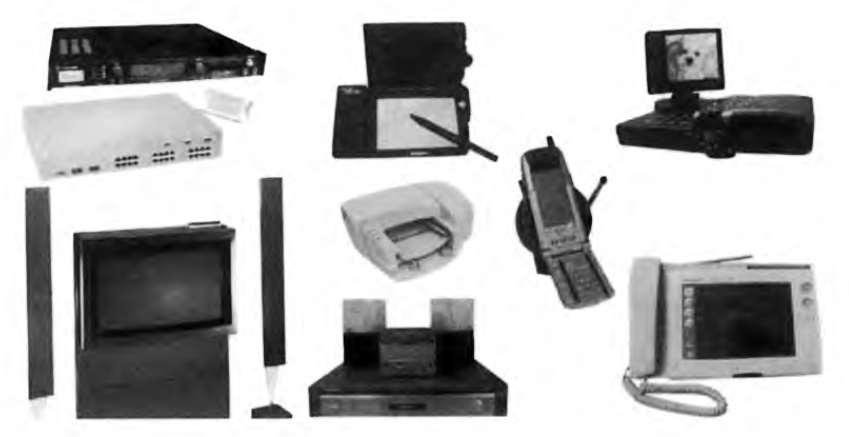
\includegraphics[width=0.5\textwidth]{Figuras/systems_embedded.PNG}
              \legend{Fonte: \cite{Li:2003:RCE:829584}}
            \end{figure}
    \par
    Uma definição geral para sistemas embarcados: são sistemas que realizam uma função dedica e possuem a integração de hardware e software fortemente acoplados, geralmente são uma parte específica de um sistema maior \cite{Li:2003:RCE:829584}.
    % microcontroladores e microprocessadores
    
    % Sistemas de tempo real e tolerancia a falha
    

    \subsection{IoT}
    \par
    A possibilidade de comunicação entre objetos de uso cotidiano do ambiente real com a internet referência o termo IoT, quando um objeto está conectado a rede de computadores e passa a transmitir informações de seu funcionamento ou estado, tal objeto passa a ser denominado de objeto inteligente \cite{iot2016}.
    \par
    De acordo com \citeauthor{iot2017}, o conceito de IoT não é novo, pois desde os passos iniciais da internet ja se pensava em formas de traçar a comunicação entre objetos do dia a dia com a internet. Com os avanços de sistemas embarcados o desenvolvimento de uma infinidades de padrões e protocolos para a integração de WSN tornaram IoT uma realidade.
    \begin{figure}[H]
              \caption{\label{fig:iot}{Internet of Things.}}
              \centering
              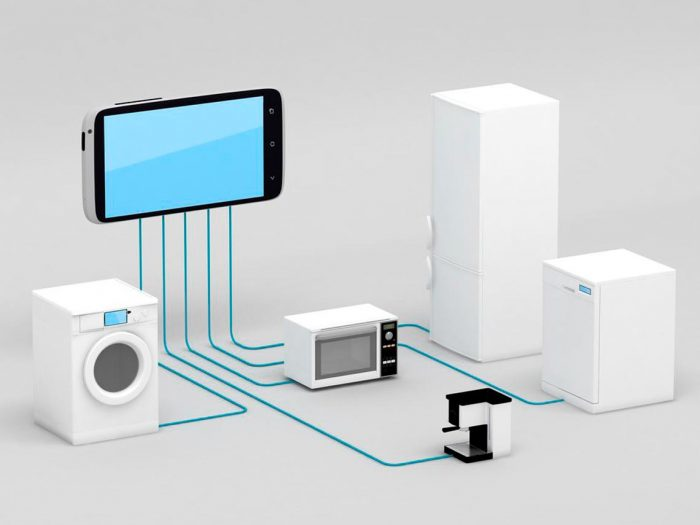
\includegraphics[width=0.5\textwidth]{Figuras/iot.png}
              \legend{Fonte: \cite{imgIot}}
        \end{figure}
    \par
    A \autoref{fig:iot} representa bem o cenário que IoT proporciona, na imagem é possível notar que todos os objetos estão conectado por uma espécie de cabo azul, mas isso é so uma representação, essa conexão também pode ser através de conectividade sem fio. Ainda sobre a imagem, o \textit{smartphone} tem um papel interesante, pois ele está sendo o encarregado de mostrar as informações enviadas pelos objetos para o usuário.
    % relação de iot com sistemas embarcados
    
\section{Comunicação Sem Fio}
    \par
    A medida que os elétrons se movimentam ondas eletromagnéticas são criada no espaço, essas ondas são medidas de acordo com suas oscilações e chamadas de frequência (Hertz), o comprimento dessa onda é medido pela distância de dois pontos máximos ou dois pontos minímos seguidos \cite{tenenbaum2002}.
    \par
    Segundo \citeauthor{tenenbaum2002} ao colocar uma antena em um circuito elétrico apropriado pode-se  transmistir e receber ondas eletromagnéticas, a comunição sem fio é baseada nisso.
    
    \subsection{Transmissão por rádio}
        % o que é 
        
        \par
        A transmissão de dados por rádio pode acontecer de duas maneiras: não-direcional e direcional  \cite{torres2001}.
        
        \begin{itemize}
        \item{Não-Direcional: }
        Quando a transmissão é feita pela forma não-direcional, a frequencias são emitidads em todas as direções e qualquer antena localizada na região de alcance das ondas de rádio podem captar os dados \cite{torres2001}, isso pode ser visto na \autoref{fig:nao_direciona}.
            \begin{figure}[H]
              \caption{\label{fig:nao_direciona}{Transmissão não-direcional.}}
              \centering
              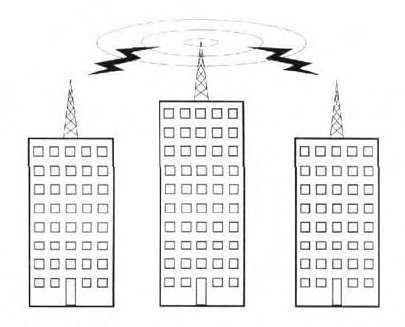
\includegraphics[width=0.5\textwidth]{Figuras/transmissao_radio_nao_direcional.PNG}
              \legend{Fonte: \cite{torres2001}}
            \end{figure}
        \par
        A  \autoref{fig:nao_direciona} mostra que as ondas de radio são emitidas em todas as direções e que qualquer antena/recepetor que estiver no alcance pode receber os dados do emissor.
        
        \item{Direcional: }
        A transmissão no sistema direcional necessita que os aparelhos transmissores e receptores estejam apontando um na direção do outro para que haja comunicação, sem contar que não pode ter obstaculos entre eles senão dificulta a transmissão \cite{torres2001}. A \autoref{fig:direcional} exemplifica o funcionamento dessa forma de transmissão.

        \begin{figure}[H]
              \caption{\label{fig:direcional}{Transmissão direcional.}}
              \centering
              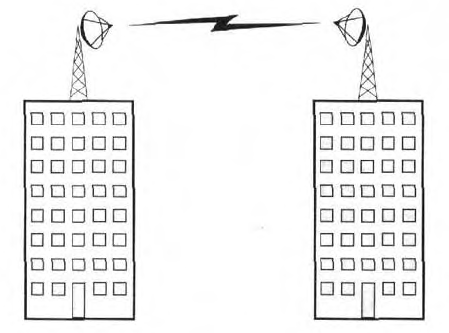
\includegraphics[width=0.5\textwidth]{Figuras/transmissao_radio_direcional.PNG}
              \legend{Fonte: \cite{torres2001}}
        \end{figure}
        \par
        De outro modo a \autoref{fig:direcional} mostra que o primeiro transmissor dever estar direcionado para a direcção do segundo trasmissor, e assim dever acontecer com o segundo transmissor também.
        \end{itemize}    
\section{Localização}
\par
Segundo \citeauthor{rfid2009review}, as informações situacionais de pessoas ou objetos têm um papel muito importante nas aplicações, dessa forma é possível saber a posição dos objetos ou pessoas para assim fazer um monitoramento ou utilizar para várias outras aplicações. Essas informações podem ser obtida através de sistemas de posicionamento, que podem ser classificados dependendo do ambiente, podendo ser destinada a ambientes internos ou externo. Esta seção aborda alguns dos tipos de sistemas de localização.
    \subsection{GPS}
    \par
    GPS é um sistema de posicionamento global implementado pelo programa NAVSTAR \textit{(Navigation System Timing and Ranging)}, iniciado no ano de 1973. Era mantido pela divisão de sistema espacial dos Estados Unidos e era destinado apenas para uso militar \cite{gpsEduardo2005}.
    \par
   O principal objetivo do uso de GPS é determinar as coordenadas espaciais de pontos referentes a um sistema mundial, para isso o sistema faz uso de distâncias entre quatros satélites, a posição do receptor é calculada a partir dos sinais recebido pelos satélites \cite{gpsEduardo2005}.

   \begin{figure}[H]
              \caption{\label{fig:satelites}{Constelação de Satélites.}}
              \centering
              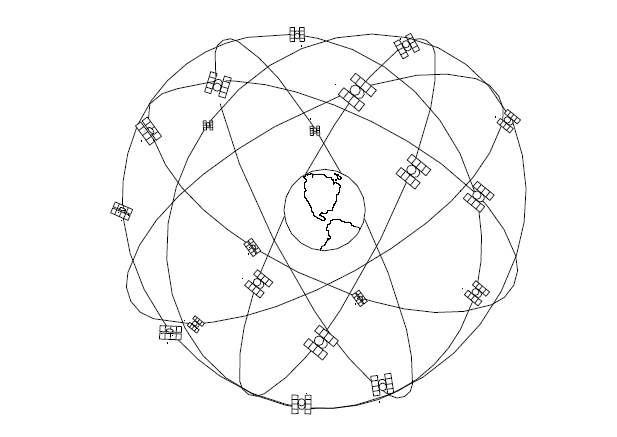
\includegraphics[width=0.5\textwidth]{Figuras/gps_satelites.PNG}
              \legend{Fonte: \cite{gpsEduardo2005}}
        \end{figure}
        \par
        A  \autoref{fig:satelites} mostra a movimentação dos satélites em torno da Terra para assim enviar sinais para os receptores que por sus vez interpretam esses sinais resultando em seu posicionamento na Terra.
 
    \subsection{WLAN}
    \par
    A localização em ambientes indoor utilizando WLANs pode ser feita com a RSSI, \textit{Angle of Arrival} (AOA), ou \textit{Time Difference of Arrival} (TDOA) \cite{wifiFernandes}. Os dispositivos devem possuir conectividade sem fio para que seja possível saber seu posicionamento no ambiente. A função que permite a utilização de RSSI está disponível em todas as interfaces 802.11 \cite{Wlan2012}.
    
    \par
    Entre as inúmeras maneiras de localizar dispositivos em ambientes fechados utilizando WLANs, algumas são: 
    \begin{itemize}
        \item {Triangulação}
        \par
        Essa forma de localizar faz uso de AOA, que seria computação dos ângulos a múltiplos ponto de acesso, o resultado disso é uma interceptação que resulta na provável localização, isso pode ser visto na \autoref{fig:triangulacao} \cite{wifiFernandes}. 
           \begin{figure}[H]
              \caption{\label{fig:triangulacao}{Triangulação.}}
              \centering
              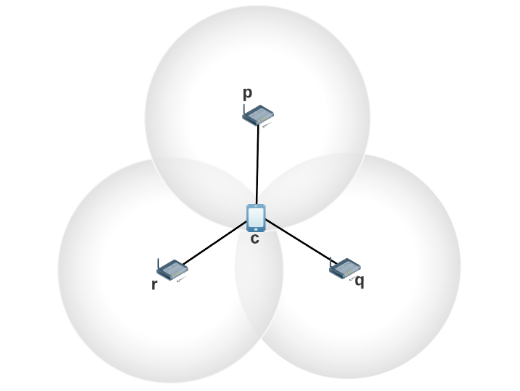
\includegraphics[width=0.5\textwidth]{Figuras/triangulacao.PNG}
              \legend{Fonte: \cite{wifiFernandes}}
        \end{figure}
        \item {Trilateração: }
        \par 
       Utilizando propriedades geométricas essa técnica faz cálculos entre múltiplos pontos de acesso para assim obter a posição do dispositivo \cite{wifiFernandes}.
        \begin{figure}[H]
              \caption{\label{fig:trilateracao}{Trilateração.}}
              \centering
              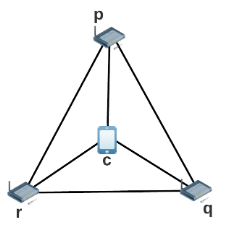
\includegraphics[width=0.5\textwidth]{Figuras/trilateracao.PNG}
              \legend{Fonte: \cite{wifiFernandes}}
        \end{figure}
       \par
        Na \autoref{fig:trilateracao} é mostrado que há uma a comunicação entre os pontos de acesso para assim poder efetuar os cálculos, esses cálculos são uma forma de saber a TDOA para assim estimar a posição do objeto \cite{wifiFernandes}.
        
        \item {Reconhecimento de padrões }
        \par
        O RSS é o principal requisito dessa técnica, em que é feita medições prévias para fazer uma comparação com os dados do banco de dados. Inicialmente é necessário uma fase em que é feita a calibração para se obter o mapa de assinatura \cite{wifiFernandes}.
        
        \par
        O mapa de assinatura é basicamente dados do banco que representam a coleção das medidas de RSSI em diferentes locais para todos os pontos de acesso no ambiente \cite{wifiFernandes}. Na \autoref{fig:fingerprinting} é mostrado seu funcionamento, onde cada ponto de acesso se comunica com o servidor para assim fazer uma comparação com os dados do mapa de assinatura.
         \begin{figure}[H]
              \caption{\label{fig:fingerprinting}{Reconhecimento de padrões.}}
              \centering
              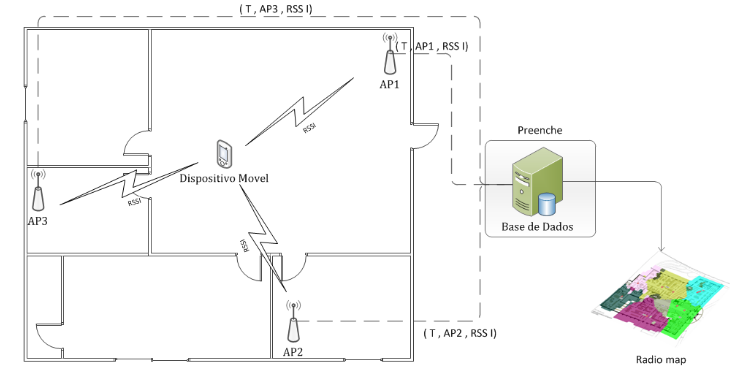
\includegraphics[width=0.9\textwidth]{Figuras/fingerprinting.PNG}
              \legend{Fonte: \cite{wifiFernandes}}
        \end{figure}
    \end{itemize}

    \subsection{RFID}
    \par
    Nessa subseção estaremos mostrando a técnica de localização com RFID utilizada no sistema \textit{LocAlizatioD iDentification based on dynaMic Active Rfid Calibration} (LANDMARC) proposto por \citeauthor{landmarc}, visto que esse sistema é citado na grande maioria das fontes que retratam a utilização de RFID para localizar objetos em ambientes fechados.
    
    \par
    O LANDMARC faz uso de tags RFID ativas para determinar o local das tags que serão localizadas, essas tags ativas são colocadas em pontos já conhecidos pelo sistema e servem como pontos de referência e assim diminuir o número de leitores e ter uma melhor precisão no ambiente \cite{RFIDapplicationsTechniques}.
    
    \par
    Através das tags ativas é possível se obter informações com relação a intensidade do sinal, essa informação é utilizada para calibrar a distância para as tags de rastreio por meio de uma soma com o peso atribuído as tags de referências mais próximas, é importante resaltar que a precisão dos resultados depende da forma que as tags de referência são posicionadas \cite{RFIDapplicationsTechniques}.
    
    \begin{figure}[H]
              \caption{\label{fig:landmarc2a}{LANDMARC.}}
              \centering
              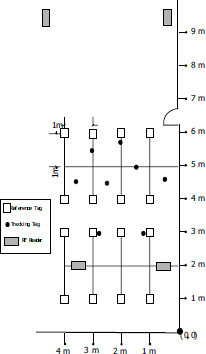
\includegraphics[width=0.4\textwidth]{Figuras/landmarc2a.png}
              \legend{Fonte: \cite{landmarc}}
        \end{figure}
    \par
    Na \autoref{fig:landmarc2a} mostra a aplicação sendo utilizada em um ambiente real por \citeauthor{landmarc}, em que os retangulos cinzas são leitores RFID, os retangulos brancos são tags de refências e os pontos pretos são tags a serem localizadas, e dessa forma o sistema calcula as coordenadas dos objetos.
\begin{comment}    
    \subsection{Sistemas de Localização }
     \begin{itemize}
        \item{LANDMARC}
        \item{RADAR}
        \item{SpotON}
     \end{itemize}
\end{comment}    
\section{Algoritmos de Localização indoor}
Nesta seção serão abordados alguns dos algoritmos que já foram utilizados para localização em ambientes indoor.
    \subsection{Multilateração}
    A multilaterção estima a coordenadas do nó de destino a partir das distâncias do nó de destino para o nó de refrência que possui coordenadas conhecidas, é o mesmo que ocorre na trilateração, porém a multilateração pode-se utilizar 2,3 ou n nós de referências, é um método utilizado para suprir a trilaterção. A inserção de mais nós tem por finalidade aumentar a precisão e diminuir a região de incerteza \cite{rfid2009review}.
    \par
    Segundo \citeauthor{rfid2009review} os calculos são execultados da seguinte forma, havendo \textit{n} nós de referência, que serão repesentado por $R_k$,  $k = \left[ 1, 2, ... , n \right] $ com suas coordenadas ja conhecidas $( x_k, y_k )$, $T$ representando o nó alvo com coordenadas desconhecidas $(x,y)$, podemos estimar utilizando a fórmula da distância da geometria analítica
    
    $\left \{ \begin{array}{c}
        r_1^2 = (x - x_1 )^2 + (y - y_1)^2  \\
        r_2^2 = (x - x_2 )^2 + (y - y_2)^2  \\
        ...  \\
        r_n^2 = (x - x_n )^2 + (y - y_n)^2 
   \end{array} \right.$
    \par 
    Depois subtraímos cada uma das equações a partir da primeira para denotar $b_{i1}= \frac{1}{2}(x_1^2 - x_i^2 + y_1^2 -y_i^2 + r_i^2 - r_1^2)$, sendo que $i = [2,3, ..., n]$ e em seguida linearizamos o sistema
    
    $\left \{  \begin{array}{c}
        b_{21} = x(x_1 - x_2) + y(y_1 - y_2)  \\
        b_{31} = x(x_1 - x_3) + y(y_1 - y_3)  \\
        ...  \\
        b_{n1} = x(x_1 - x_n) + y(y_1 - y_n)
   \end{array} \right.$\\
     que também pode ser escrito no formato de matriz $b = AX$. Esse algortimo requer pouca computação e está em uso em muitos sistemas de localização.    

    \subsection{Inferência Bayesiana}
  Segundo \citeauthor{bayesian2001} a inferência bayesiana é dedução estatística através de evidências ou analíse observatória para que a inferência de uma hipótese possa vir a ser verdadeira, e no caso da localização de um dispositvo isso pode ser realizado utilizando RSS entre o nó de destino e os pontos de acesso.


    \begin{figure}[H]
              \caption{\label{fig:bayesian}{Rede Bayesiana}}
              \centering
              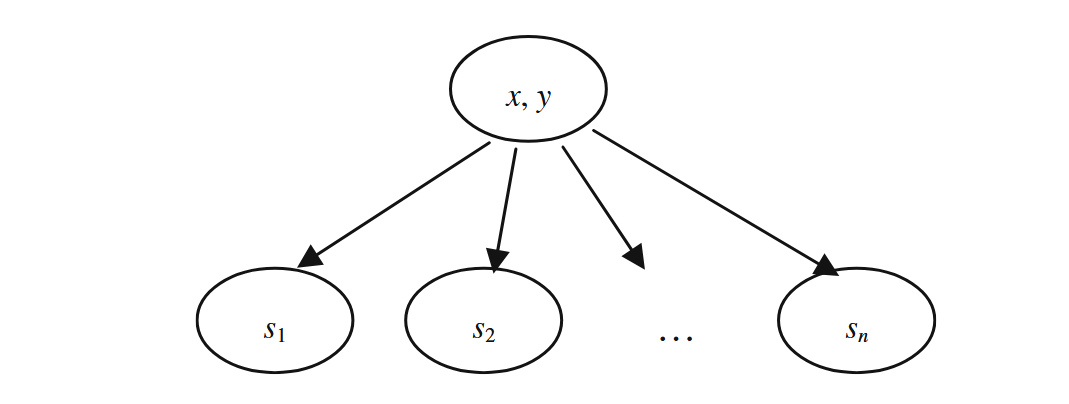
\includegraphics[width=0.4\textwidth]{Figuras/bayesian_network.PNG}
              \legend{Fonte: \cite{rfid2009review}}
        \end{figure}

        Na \autoref{fig:bayesian} temos uma representação de uma rede bayesiana para localização estacionária, onde as coordenadas $(x,y)$ representam o nó que será localizado e o $S_i$, $i=1,...,n$ são uma série de intesidades de sinais trasmitidas ou recibidas pelos pontos de refências do sistema, como nesse sistema as probabilidade de $S_i$ são idependentes e não interferem uma na outra dizemos que há uma satisfação em relação a condição de Markov \cite{rfid2009review}.
        \par
        \citeauthor{rfid2009review} afirma que a localização do dispositvo alvo pode ser obtida atravé da fórmula recursiva 
        $P((x,y) | s_1, s_2, ..., s_n) = \alpha P(s_n | (x,y)) \times P((x,y) | s_1,s_2, ...,s_{n-1})$, nessa expressão $\alpha$ é um fator de nomalização para que a soma da probabilidade posterior, no caso a primeira parte da expressão $P((x,y) | s_1, s_2, ..., s_n)$ seja uma e $(s_n | (x,y))$ calcule a probabilidade da RSSI dada para a localização do dispositivo, é importante resaltar que essa é uma expressão para localizar alvos estáticos. 
        
    \subsection{K-Nearest-Neighbor}
    Os algoritmos de vizinhaça ou no caso de \textit{nearest-neighbor} tem uma abordagem bem simples que envolve utilizar os nó ja classificados para classificar os novos nós a partir da medida de similaridade \cite{knn-3dLAN}, de outro modo, utilizar-se dos seus vizinhos para assim obter suas coordenadas com os cálculos baseados em RSS \cite{rfid2009review}.

    \par
    algumas das metricas abordada por \citeauthor{knn-3dLAN} são:

    \begin{itemize}
    \item Distância Euclidiana 
      \par
      $Dist(r,s) =  \sqrt{(x_r - x_s)(x_r - x_s)^\prime}$
    \item Padronização da Distância Euclidiana
      \par 
      $Dist(r,s) =  \sqrt{(x_r - x_s)D^-1(x_r - x_s)^\prime}$
    \item Distância de Mahalanobis
      \par
        $Dist(r,s) =  \sqrt{(x_r - x_s)V^-1(x_r - x_s)^\prime}$
    \item Distância de Manhattan
      \par
      $Dist(r,s) = \sum_{j=1}^{n} |x_{rj} - x_{sj}|$
    \item Distancia de Minkowski
      \par
      $Dist(r,s) = \sqrt[p]{\sum_{j=1}^{n}|x_{rj} - x_{sj}|^p}$

    \end{itemize}
   \par
   \citeauthor{rfid2009review} faz mostra uma outra abordagem para calcular as coordenadas do alvo obtidos a partir do sistema a seguir:
   
   $\left \{ \begin{array}{c}
        x= \sum_{i=1}^{k}w_{i}x_{i}   \\
        y= \sum_{i=1}^{k}w_{i}y_{i}  
   \end{array} \right.$ \\
    nesse sistema o $k$ representa a quantidade de vizinhos, $(x_i,y_i)$ são as coordenadas dos pontos de refências vizinhos e $w_i$ os pesos desses pontos,o cálculo dos pesos é feito a partir da diferençã de RSSI entre os pontos de refências e o alvo e as fórmulas para tal são:
    \begin{itemize}
        \item $w_i = \frac{1 / \sum_{j=1}^{m}|s_{ij} - s_{j}|}{\sum_{j=1}^{k} (1/ \sum_{j=1}^{m}|s_{ij} - s_{j}|)}$ 
        
        \item  $w_i = \frac{1 / \sqrt{\sum_{j=1}^{m}(s_{ij} - s_{j})^2}}{\sum_{j=1}^{k} (1/ \sqrt{\sum_{j=1}^{m}(s_{ij} - s_{j})^2})}$ 
    \end{itemize}$\\$
    nas expressões de $w_i$, dizemos que $s_j$ e $s_{ij}$, $j =1, ..., m$ represetam  RSSI dos respectivos ponto de referências e nó alvo que será localizado. 
    
    \subsection{Proximidade}
    A técnica de Proximidade, segundo \citeauthor{rfidProximity} baseia-se no princípio de que se o alvo está no alcance de uma antena ou leitor, sua localização será a mesma que a da antena e se o alvo está no alcance de duas ou mais antenas, a localização dada é aquela cujo possui a intensidade do sinal mais forte. Já para \citeauthor{rfid2009review} quando o alvo esta no alcance de dois ou mais receptores, utiliza-se o calculo de centroíde para estimar a localização.
    
    %\subsection{Aprendizado Baseada em Kernel}
\section{Modelagem de Sistemas}
    \subsection{UML - \textit{Unified Modeling Language}}
    O UML(em português Linguagem de Modelagem Unificada ) é uma linguagem cujo principal papel é a construção, visualização e documentação de projetos de sistemas. Surgiu na década de 90, tendo em vista que havia a necessidade de uma linguagem para modelagem que funcionasse como uma norma e fosse aceita e utilizada pela indústria, ambientes acadêmicos e de investigação \cite{uml}.
    \par
    Na UML é possível agrupar elementos e relaciona-los de maneira lógica ou estrutural, isso é o conceito de diagramas. Os elementos tem um papel importante nos modelos, eles estarão organizados de acordos com a função desempenhada no sistema, podendo representar componetes do sistema, usuário, interfaces \cite{uml}.
    
    \begin{figure}[H]
              \caption{\label{fig:uml-elementos}{Elementos UML}}
              \centering
              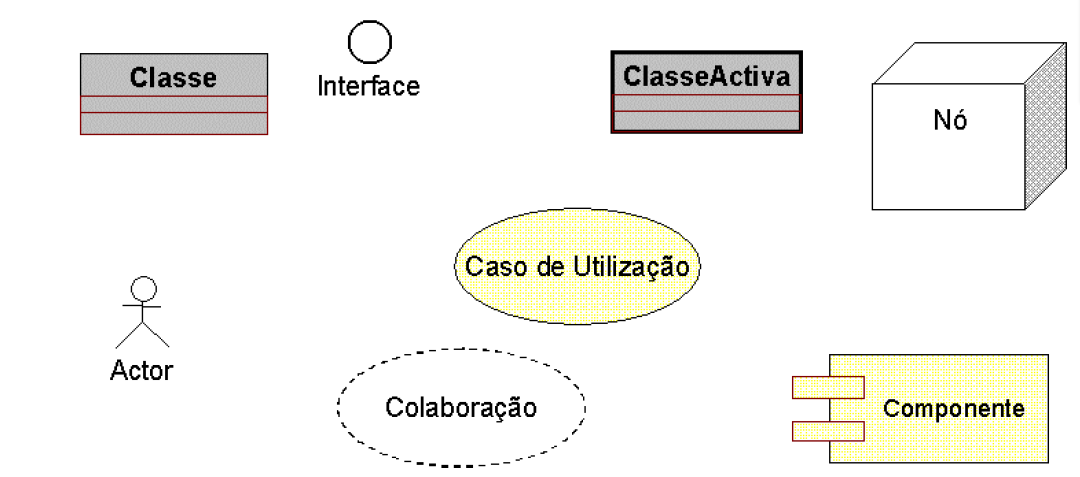
\includegraphics[width=0.9\textwidth]{Figuras/uml1.PNG}
              \legend{Fonte: \cite{uml}}
        \end{figure}
    \par
    Na \autoref{fig:uml-elementos} está um resumo de alguns elementos básicos que é utilizados em modelos de projetos de software, esses compontes por mais que sejam básicos, possibilitam a representação de vários componentes em um projeto.
    \par
 
    \subsection{Redes de Petri}

% ----------------------------------------------------------
% Revisão de Literatura
% ----------------------------------------------------------
\chapter{TRABALHOS CORRELATOS}
\label{chapter:correlatos}
Este capítulo tem como objetivo apresentar os principais trabalhos relacionados com o sistema proposto neste trabalho, exaltando as diferenças e contribuições para o método proposto neste trabalho. Os trabalhos em específico abordados utilizam tag RFID ou referenciam sistemas que fazem uso de tal ferramenta para localizar e identificar objetos em ambientes fechados: An indoor localization mechanism using active RFID tag \cite{mechanismRFID2006}, Real-Time Locating Systems Using Active RFID for Internet of Things \cite{realtimeRFID2016}, Object localization using RFID \cite{localization2010} e RFID localization algorithms and applications-A review \cite{rfid2009review}.

\section{An indoor localization mechanism using active RFID tag}
O trabalho de \citeauthor{mechanismRFID2006} faz uma análise do método utilizado no sistema LANDMARC e depois propõe uma melhoria para o método. O LANDMARC é um sistema de localização que faz uso de tag de referência. As tags de referência são tags ativas colocadas em pontos fixos que servem como pontos de referência para o sistema e calibração da localização, esse sistema utiliza tags ativas visando diminuir a quantidade de leitores RFID para baratear o sistema.

%Funcionamento do landmarc
\par
Segundo \citeauthor{mechanismRFID2006} o LANDMARC funciona da seguinte maneira: primeiro os leitores detectam as tags de referências que estão no seu alcance, após isso é concedido ponderação as tags de referências de acordo com RSS, sendo valor mais alto para as mais próximas. O passo seguinte é realizar o cálculo da distância euclidiana na RSS entre uma tag de rastreamento e uma tag de referência e quanto menor o resultado mais próximo da tag de referência. Por fim o sistema escolhe k tags de referências com os menores valores no resultado do cálculo e obtém a localização da tag de rastreamento por meio da $(x,y) = \sum^k_{i=1}w_i(x_i,y_i), w_j=\frac{\frac{1}{E_i^2}}{\sum_{i=1}^k\frac{1}{E^2_i}}$. 
%Melhoria proposta
\par
\citeauthor{mechanismRFID2006} mostra que LANDMARC possui alguns problemas, sendo efetuando cálculos desnecessários durante a escolha das tags vizinhas e comparação de valores RSS de leitores que não estão no alcance da tag alvo. Para melhorar o sistema \citeauthor{mechanismRFID2006} propõe a utilização apenas dos leitores RFID  e tags de referência que alcançam o alvo, sendo que o número de leitores e das tags de referência tem que ser maior que 3, pois depois o método consiste em utilizar a técnica de Triangulação.
%Comparação com o método proposto
\par
O método utilizado por \citeauthor{mechanismRFID2006} tem objetivo de ter alcançar grande precisão no posicionamento em relação ao ambiente, já o método proposto neste trabalho tem objetivo de saber exatamente a sala que os objetos estão, tendo em vista que o ambiente possui inúmeras salas. Entretanto essa aplicação para posicionamento na sala pode ser acrescentado e estudada em trabalhos futuros.

\section{Real-Time Locating Systems Using Active RFID for Internet of Things}
O trabalho de \citeauthor{realtimeRFID2016} propõe um sistema de localização em tempo real, o iLocate é mais um sistema que faz uso de tags ativas, e  utilizar-se de ZigBee para assim assegurar que a transmissão de dados a longa distância seja garantida. 
\par
O sistema proposto por \citeauthor{realtimeRFID2016} inicialmente aplica uma técnica de \textit{fingerprinting} que seria uma técnica equivalente ao reconhecimento de padrões abordada em \autoref{subsection:wlan}, iniciando com uma leituras breve de RSSI e implantação de tags de referências no mapa de interesse, seguindo para o armazenamento das leituras no banco de dados e construção de uma matriz com dados de RSSI. 
\par 
O iLocate conta com um refinamento para ter uma localização mais precisa, que funciona criando tags de referência virtuais que também utiliza a técnica de \textit{fingerprinting} para comparar com a reais. Outro recurso encontrado no iLocale é a comunicação tag-tag em que possibilita a troca de mensagens entre tags de referências que estão no mesmo intervalo de trabalho \cite{realtimeRFID2016}.
\par
A utilização de uma base de dados por \citeauthor{realtimeRFID2016} é um recurso que também será utilizado no sistema proposto neste trabalho, por mais que os dados armazenados sejam diferentes o banco de dados terá função importante.

\section{Object localization using RFID}
Na pesquisa de \citeauthor{localization2010} é proposto um método de localização que permite estimar a posição de objetos com rapidez e velocidade utilizando a variação dos níveis de potência dos leitores, o método ainda faz uso de tags de referência para auxiliar na localização das tags que serão rastreadas.

\par
O método proposto por \citeauthor{localization2010} foi aplicado em uma sala cuja as dimensões são 2m x 3m. A região que assemelha a um retângulo foi dividida em oito sub-regiões de tamanho iguais e denominadas de setores, em seguida cada setor foi dividido em quatro regiões de tamanho iguais chamados de quadrantes.

\par
Depois de fazer a divisão do ambiente é passado para inserção de tags de referências em cada quadrante, essas tags de referência são utilizadas inicialmente para calibrar os leitores RFID com uma relação de potência em contraste com distância. Por fim é utilizados algoritmos que ficam variando o nível de potência do leitor, esses algoritmos podem iniciar a variação da potência do menor para maior até alcançar um nível mínimo para localizar o objeto ou podendo utilizar uma variação da potência do maior para o menor \cite{localization2010}.

\par
O método \citeauthor{localization2010} diferencia-se do método proposto no caso de buscar uma localização e posicionamento preciso em ambiente fechado, o que não se torna uma prioridade para o método proposto neste trabalho.


\section{RFID localization algorithms and applications-A review}
O artigo de \citeauthor{rfid2009review} tem uma abordagem diferente dos trabalhos anteriores, não propondo nenhum método de localização mas mostrando as aplicações existentes, revisando algoritmos de localização indoor e potenciais da localização de RFID.
\par
RFID pode ser empregado em várias aplicações, de acordo com \citeauthor{rfid2009review} RFID é utilizado no porto de Cingapura para posicionar os contêiner, na saúde para localização de pacientes, suprimentos e equipamentos  e também na gestão de material de construção permitindo monitoramento do andamento e status da construção.
\par
No artigo é realizado uma revisão dos algoritmos de localização classificando-os em dois grupos, o grupo que calibra a distribuição do sinal de radiofrequência e depois estima a posição do objeto e o segundo grupo que calculam diretamente a posição do objeto utilizando dados de RSSI. Dentro do primeiro grupo encontramos os algoritmo de multilateração e inferência bayesiana, já no segundo grupo estão os algoritmos de aprendizados em proximidade e de proximidade \cite{rfid2009review}.
\par
O artigo de \citeauthor{rfid2009review} teve grande contruibuição para esta pesquisa, solucionando duvidas e abordando assuntos importates para utilização de RFID e sistemas de localização.



% ----------------------------------------------------------
% Detalhes de Desenvolvimento do Projeto
% ----------------------------------------------------------
\chapter{MÉTODO PROPOSTO}

\label{chapter:metodo}
Este Capítulo tem o objetivo de descrever a metodologia proposta neste trabalho, visando localizar e identificar objetos em ambientes confinados utilizando leitores e etiquetas passivas RFID, para gerenciamento e controle de bens.

\section{Visão geral do método}
O método consiste em um sistema que localiza qualquer objeto que tenha uma etiqueta RFID passiva fixada em seu corpo, as etiquetas serão localizadas e identificadas a medida em que transitam de uma sala para outra em um edifício. A localização e identificação é feita por meio de leitores RFID e controladores colados próximos a porta e os leitores devem ler tags que passam pela porta.
\par
Cada leitor RFID junto ao controlador será responsável por uma sala, portanto qualquer etiqueta lida por aquele leitor ocasionará nas ações referentes a mesma sala. As ações poderá ser de atualização sobre a localização do objeto ou informando que o objeto está em transição para outra sala no edifício.
\begin{figure}[H]
              \caption{\label{fig:modelo}{Modelo Proposto}}
              \centering
              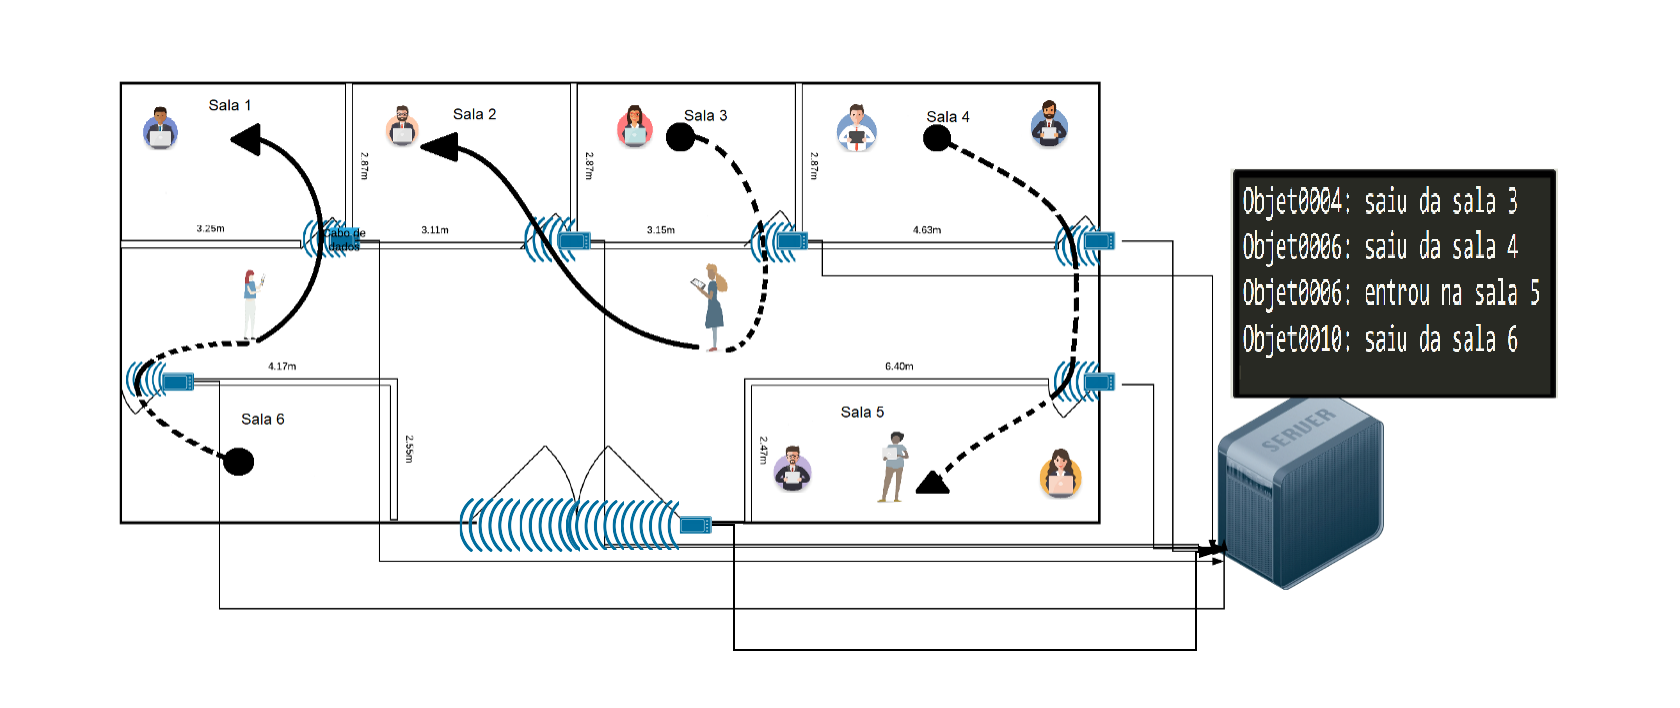
\includegraphics[width=1.1\textwidth]{Figuras/bigpicture.png}
              \legend{Fonte: Própria}
        \end{figure}
\par
Na \autoref{fig:modelo} é possível notar que há um dispositivo acoplado próximo a porta de cada sala, esse dispositivo cotém o leitor RFID, esse dispositvo será encarrecado de consultar um servidor para assim tomar decisões do que será feito com o status do objeto, cada objtetos possui uma tag RFID fixada nele e quando passar pela porta o leitor identifica o objeto e altera sua as informações sobre sua localização.

\par
O método proposto consiste basicamente nas seguintes etapas:
\begin{enumerate}
    \item Identificação dos objetos rastreáves
    \item Monitoramento dos objetos rastreáves
    \item Localiazação do objetos em ambiente indoor
    \item Configuração do tempo para alertas
\end{enumerate}
\section{Identificação dos objetos rastreáveis}
Antes de qualquer passo é necessário a identificação dos objetos, nessa etapa é anexadas ao objetos as etiquetas RFID e realizada uma descrição do objeto portador dessa etiqueta no sistema, para que ao entrar e sair das salas do edifício além de fornecer a localização do objeto também seja possível ter detalhes sobre aquele objeto, dessa forma se objeto tiver uma registro local isso irá constar na descrição do objeto. Essa etapa pode ser considerada como a fase de cadastro.

\section{Monitoramento e Localização dos objetos rastreáveis}
O monitoramento é realizado pelos sensores RFID que estará em cada porta das salas do prédio e será responsável por enviar mensagens para o servidor sobre as ocorrências da sala para que medidas sejam realizadas.
\subsection{Fluxo de execução do método em cada sala}
Os dispositivos de cada sala terão o seguinte fluxo de execução apresentado na \autoref{fig:fluxograma}, o fluxo exemplifica as tarefas que cada dispositivos executarão. Neste fluxograma os retangulos represetam processos e retângulos com bordas duplas processos pré-definidos, os losangos represetam as tomadas de decisões, os icones com bordas curvas para o mesmo lado representam operações nos dados do sistema e o ícone com bordas curvas opostas represetam o inicio do fluxo.
\begin{figure}[H]
              \caption{\label{fig:fluxograma}{Fluxograma de cada sala}}
              \centering
              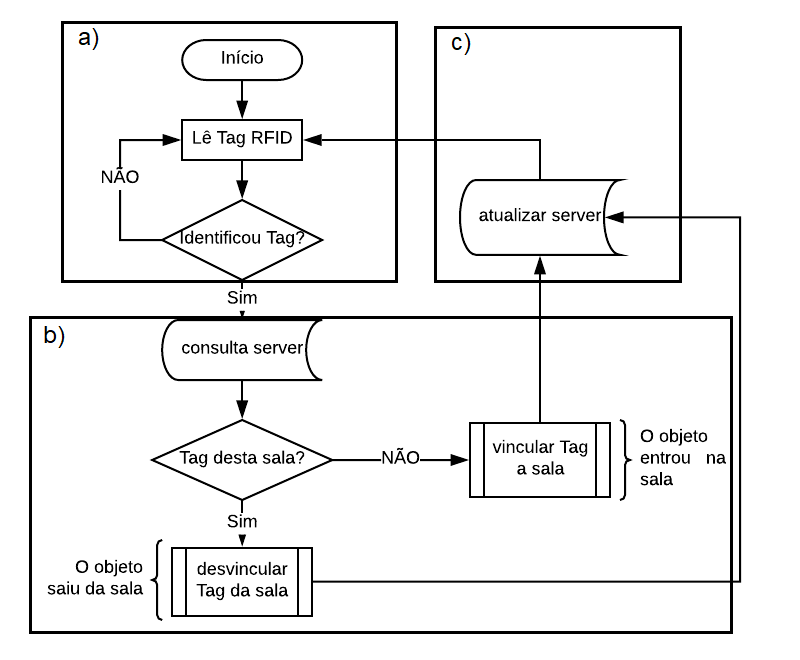
\includegraphics[width=1\textwidth]{Figuras/fluxograma.png}
              \legend{Fonte: Própria}
\end{figure}
\par
O fluxograma é separado em três módulos: \textbf{a}, \textbf{b} e \textbf{c}. O modulo \textbf{a} é onde é realizado o monitoramento da da sala, realizando leituras dos objetos que entram e saem da sala, no módulo \textbf{b} é o onde serão tomadas as decisões referente a etiqueta anexada ao objeto lida naquele momento, verificando se a etiqueta está ou não localizada naquela sala e processando as alterações necessárias. O módulo \textbf{c} é o último processo que atualiza as informações do servidor para que os dados consultados sejam iguais para todos. 
\subsection{Localização dos objetos}
Os objetos serão localizado no sistema baseado nos algoritmos de proximidade, ou seja, a partir do momento em que o leitor RFID identifica uma etiqueta, esse objeto terá a localização referente à aquele leitor, nesse sistema os leitores irão representar salas, portanto a localização indicará que o objeto estará na sala cujo o leitor que realizou a leitura representa.
\par
O sistema conterá um servidor que possui a função de tratar problemas relacionados a leituras de uma mesma etiqueta mais de uma vez, o papel do servidor é de grande importância também sendo utilizado para consultar informações referentes aos objetos.

\section{Alertas}
Para um melhor gerenciamento dos objetos, o sistema conta com alertas para que caso um objeto inicie uma transição para outra sala e nesse trajeto o objeto não entre em nenhuma sala excedendo um tempo determinado, um alerta é gerado informado que o objeto não entrou em nenhuma sala do edificio até o momento da geração do alerta.
\par
Um tempo padrão deve ser configurado para os alertas, se um objeto excede esse tempo na transição um alerta é gerado no servidor. O tempo deve ser configurado na implatação do sistema.

\section{Conexão dos dispositivos de porta com o servidor}
A comunicação entre os dispositivos da porta com o servidor acontecerá por meio de uma WLAN, ou seja todos estarão em uma rede local e assim poderrão se comunicar, entretanto a comunicação será diretamente entre um dispositivo e o servidor, não havendo comunicação entre dois dispositivos. O Arduino nano contará com um módulo ESP8266, esse módulo possibilita a conexão com uma rede weriless 802.11 b/g/n.

\section{Modelo de Prototipação}
O protótipo é composto pelo servidor que nesse primeiro instante será um computador de propósito geral e pelo dispositivo da porta, que será um Arduino Nano ATmega168 junto ao leitor RFID RC522 e módulo ESP8266, o leitor pode ser visto na \autoref{fig:leitorRFID}, esse leitor é capaz de ler etiquetas que operam em frequências de 13,56 Mhz.
\begin{figure}[H]
              \caption{\label{fig:leitorRFID}{Leitor RFID RC522}}
              \centering
              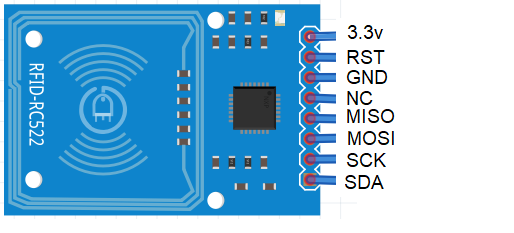
\includegraphics[width=0.7\textwidth]{Figuras/rfid_rc522.PNG}
              \legend{Fonte: Fritzing}
\end{figure}

\par
O leitor RFID utiliza a interface SPI (\textit{Serial Peripheral Interface} ) para comunicação com o Arduino, essa conexão é síncrona e é realizada por meio dos pinos  9 à 13. A prototipagem entre o Arduino e o leitor RFID segue o seguinte esquema abaixo também podendo ser vista na \autoref{fig:esq_conexoes}:
\begin{itemize}
    \item 3.3V - conectado ao pino de 3.3v no Arduino, essa conexão faz a alimentação do leitor RFID;
    \item RST - conectado ao pino 9 do Arduino;
    \item GND - conectado ao pino GND do Arduino;
    \item NC - não utiliazado;
    \item MISO - conectado ao pino 12;
    \item MOSI - conectado ao pino 11; 
    \item SCK - conectado ao pino 13;
    \item SDA - conecatado ao pino 10.
\end{itemize}
\begin{figure}[H]
              \caption{\label{fig:moduloWii}{Módulo Wifi ESP8266}}
              \centering
              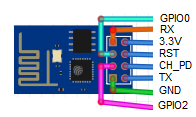
\includegraphics[width=0.6\textwidth]{Figuras/Modulo_ESP8266.png}
              \legend{Fonte: Fritzing}
\end{figure}
\par
O ESP8266 é um módulo que permite a conexão do Arduino com redes wireless 802.11 b/g/n, esse módulo pode trabalhar em dois modos tanto como ponto de acesso ou no modo STA, estação que envia e recebe dados. 
\begin{itemize}
    \item 3.3V - conectado ao pino de 3.3v no Arduino;
    \item GND - conectado ao pino GND do Arduino;
    \item GPIO0 - não conectado ;
    \item GPIO2 - não conectado ; 
    \item TX - conectado ao pino digital 2 no Arduino;
    \item RX - conecatado ao pino digital 3 no Arduino junto com dois resistores um de 220$\Omega$ e outro de 330$\Omega$ para dividir a tensão;
    \item RST - não conecatado ;
    \item CH\_PD - conecatado ao pino 3.3v mas com resistor de 10 $K\Omega$.
\end{itemize}
\begin{figure}[H]
              \caption{\label{fig:esq_conexoes}{Esquema de Conexões}}
              \centering
              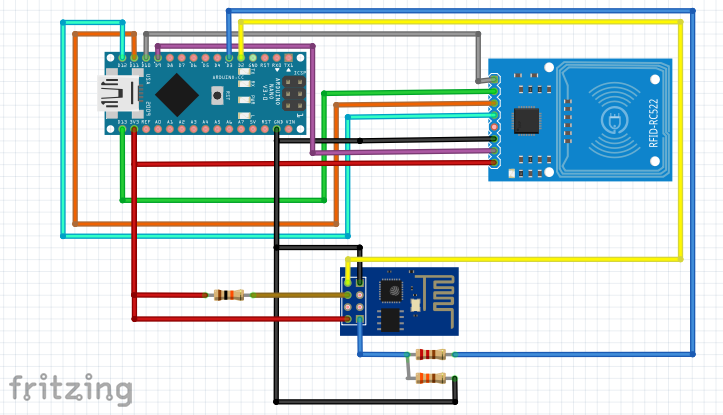
\includegraphics[width=1\textwidth]{Figuras/esquema_de_conexoes2.PNG}
              \legend{Fonte: Própria}
\end{figure}


% ----------------------------------------------------------
% Cronograma
% ----------------------------------------------------------
\chapter{CRONOGRAMA}
\label{chapter:cronograma}
\begin{table}[htbp]
  \centering
  \caption{Cronograma de atividades}
  \label{tab:cronograma}
  \begin{tabularx}{\textwidth}{|X|c|c|c|c|c|}
    \hline
    \textbf{Atividade} & \textbf{Janeiro} & \textbf{Fevereiro} & \textbf{Março} & \textbf{Abril} & \textbf{Maio} \\
    \hline
    Revisão da literatura sobre localização e identicação de objetos utilizando RFID & \(\times\) & \(\times\) & & & \\
    \hline
    Construção do prótotipo e realização de testes & \(\times\) &  \(\times\) & & & \\
    \hline
   Configuração do servidor e testes de conexões com os dispositivos & & \(\times\) & & & \\
    \hline
    Teste nas transições, adições e atualizações dos objetos & & & \(\times\) & \(\times\) &  \\
    \hline
    Finalização do prótotipo & & &  & \(\times\) & \\
    \hline
    Finalização monografia & & & & \(\times\) & \(\times\) \\
    \hline
    Apresentação final & & & &  & \(\times\) \\
    \hline
  \end{tabularx}
\end{table}

% ----------------------------------------------------------
% Resultados -- Pode vir junto com discussão
% ----------------------------------------------------------
\chapter{RESULTADOS EXPERIMENTAIS}
\label{chapter:resultados}
O presente capítulo consiste em apresentar a execução e resultado referente ao método proposto, visando avaliar de forma experimental o INEXT para identificação e localização de objeto em edifícios utilizando RFID.

\section{Planejamento e projeto dos experimentos}
Esta avaliação experimental consiste em avaliar o INEXT, tendo como questões principais a identificação e localização de objetos em ambientes confinados e então o gerenciamento dos objetos. Em virtude disso, foi definida as seguintes questões:
\begin{itemize}
    \item[QP1]: O sistema proposto consegue identificar e localizar objetos no âmbito confinado?
    \item[QP2]: O método proposto agiliza o gerenciamento dos objetos em edifícios?
    
\end{itemize}{}
\par 
Objetivando responder tais questões, foram utilizados um Arduíno Nano e um computador comunicando-se através da porta serial para simular a segunda sala, pois não disponhamos de duas placas NodeMcu, em seguida usamos um \textit{script} na linguagem Python para ler os dados da porta serial, criar um objeto JSON e enviar para o servidor, tais código estão disponíveis no repositório dentro da pasta ''prototype\_arduino''. O computador utilizado possui $4GB$ de memória RAM, processador Intel Core $i5-2500$, HD de $500GB$ e sistema operacional \textit{Windows} $7$ \textit{Professional} $64Bits$.  Os protótipos podem ser visualizados nas \autoref{fig:prototipo_arduino} e \autoref{fig:prototipo_nodemcu}. 

\begin{itemize}
    \item 3.3V - conectado ao pino de 3.3v no Arduino, essa conexão faz a alimentação do leitor RFID;
    \item RST (\textit{Reset})- conectado ao pino 9 do Arduino;
    \item GND (\textit{graduated neutral density filter}) - conectado ao pino GND do Arduino;
    \item NC/IRQ (\textit{Interrupt Request})- não utilizado;
    \item MISO (\textit{Master In Slave Out}) - conectado ao pino 12;
    \item MOSI  (\textit{Master Out Slave In}) - conectado ao pino 11;
    \item SCK  (\textit{Serial Clock}) - conectado ao pino 13;
    \item SDA/ SS (\textit{Serial Data Line/ Select Slave}) - conectado ao pino 10.
\end{itemize}    

\begin{figure}[H]
              \caption{\label{fig:esq_conexoes_arduino}{Esquema de Conexões Arduíno Nano}}
              \centering
              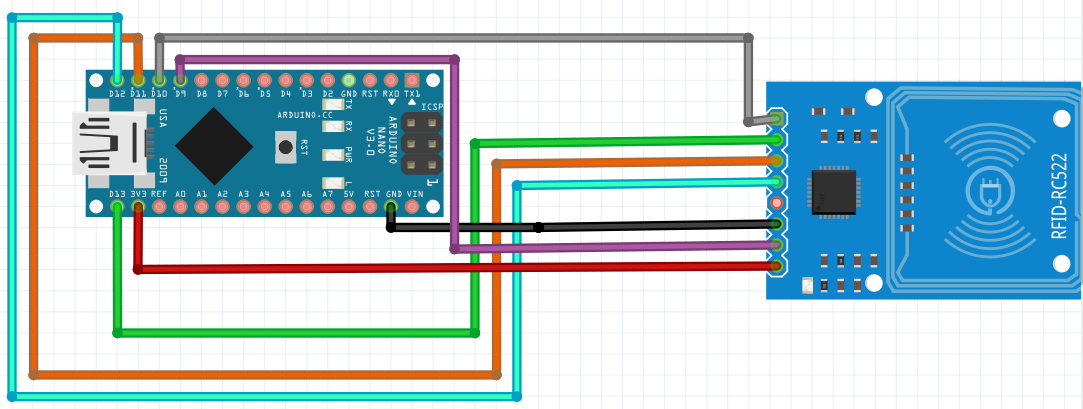
\includegraphics[width=1\textwidth]{Figuras/esquema_de_conexoes1.PNG}
              \legend{Fonte: Própria}
\end{figure}
\begin{figure}[H]
              \caption{\label{fig:prototipo_arduino}{Protótipo Arduíno Nano}}
              \centering
              \includegraphics[width=1\textwidth]{Figuras/prototype_arduino.png}            \legend{Fonte: Própria}
\end{figure}\begin{figure}[H]
              \caption{\label{fig:prototipo_nodemcu}{Prototipo NodeMcu}}
              \centering
              \includegraphics[width=1\textwidth]{Figuras/prototype_nodemcu.png}
              \legend{Fonte: Própria}
\end{figure}
\par
Para a simulação do servidor, foi utilizado um notebook com $6GB$ de memória RAM, processador Intel Core $i5-4200$, HD de $750GB$, placa de video GeForce $720M$ de $2GB$ de memória dedicada e sistema operacional \textit{Windows 10 Home Single Language}. A rede LAN utilizada foi criada através de um roteador \textit{TP-LINK} modelo $TL-WR720N$. Também foram utilizadas quatro etiquetas RFID passivas, cada uma dessas etiquetas representa um objeto diferente para a simulação.

\section{Execução dos experimentos e Análise dos Resultados}
A execução do experimento aconteceu no cenário apresentado na \autoref{fig:cenario}, como havia sido mencionado anteriormente, foi simulado duas salas e quatro objetos rastreáveis em um edifício. Foram executados os seguintes testes: (1) localização e identificação dos objetos, (2) restrição de objeto e notificação ao violar restrição e (3) gerenciamento dos objetos.
\begin{figure}[H]
              \caption{\label{fig:cenario}{Cenário de simulação}}
              \centering
              \includegraphics[width=1\textwidth]{Figuras/cenario.png}
              \legend{Fonte: Própria}
\end{figure}
\par
Após a execução dos testes, foi constatado que o INEXT consegue localizar objetos em ambientes confinados, porém o sistema não proporciona a posição real do objeto no ambiente, o sistema também foi capaz de identificar os objetos mas essa etapa ainda ocorre de maneira manual necessitando ser realizada por usuários.

\par
Os testes seguintes foram a criação de restrição para objetos e verificar se os todos usuário eram notificados quando a restrição fosse violada, o sistema foi capaz de notificar os usuários através do e-mail e na tela inicial do sistema. O ultimo teste foi a realização do levantamento de todas as salas e objetos que cada sala possui, o INEXT foi capaz de realizar essa tarefa e gerou logs para todas as operações realizadas.

%\chapter{DISCUSSÃO}

% ----------------------------------------------------------
% Conclusão
% ----------------------------------------------------------
\chapter{CONSIDERAÇÕES PARCIAIS E TRABALHOS FUTUROS}
\label{chapter:consideracoes}
Este trabalho faz uma abordagem para a construção de um sistema de localização e identificação de objetos em edifícios por meio de radiofrequência e etiquetas passivas. O real objetivo consiste em facilitar e auxiliar o gerenciamento/controle de bens em edifícios cujo possuem uma grande quantidade de salas.

\par
Para os trabalhos futuros, visando ter uma localização mais precisa sobre a localização dos objetos pode-se utilizar etiquetas ativas para auxiliar e em seguida aplicar algoritmos de RSSI, dessa forma tende-se a ter uma localizão com maior precisão no ambiente.
%\newpage
% ----------------------------------------------------------
% Referências bibliográficas
% ----------------------------------------------------------
\bibliography{main}

%---------------------------------------------------------------------
% INDICE REMISSIVO
%---------------------------------------------------------------------
%\phantompart
%\printindex
%---------------------------------------------------------------------

\end{document}

